% !TEX encoding = UTF-8 Unicode
\documentclass[xcolor=dvipsnames]{beamer}

\beamertemplatenavigationsymbolsempty
\setbeamertemplate{footline}[frame number]

\usecolortheme{rose}
\useinnertheme{default}

% packages
\usepackage{fancybox}
\usepackage{colortbl}

% language
%\usepackage{ctex}
\usepackage[applemac]{inputenc}
\usepackage[ngerman]{babel}														
\usepackage[T1]{fontenc}	
														
\usepackage{textcomp}
\usepackage{marvosym}
\usepackage{url}

\usepackage{tikz}
\usetikzlibrary{arrows.meta,positioning}
\usepackage{pgfplots}
\usetikzlibrary{shapes,decorations,positioning}
\usetikzlibrary{fit}
\usepackage[outline]{contour}
\contourlength{1.2pt}

\tikzset{
    %Define standard arrow tip
    >=stealth,
    % Define arrow style
}

\pgfplotsset{colormap/violet}

\usepackage{pdfrender}
\usepackage{comment}
\usepackage{multirow}
\usepackage{subfig}

\usepackage{mathtools}
\usetikzlibrary{shapes,arrows,snakes,calc}


\usepackage{amsmath, amssymb, amstext, amsfonts, mathrsfs, dsfont}
\usepackage[]{pict2e}
\usepackage{epstopdf}

\usepackage{multirow}
\usepackage{chngpage}

% individual macros
\newcommand{\C}{\mathbb{C}}
\newcommand{\R}{\mathbb{R}}
\newcommand{\Q}{\mathbb{Q}}
\newcommand{\Z}{\mathbb{Z}}
\newcommand{\N}{\mathbb{N}}
\newcommand{\Spp}{\mathbb{S}^n_{++}}
\newcommand{\dom}{\mathrm{dom}}
\newcommand{\epi}{\mathrm{epi}}
\newcommand{\inter}{\mathrm{int}}

\newcommand{\Rn}{\mathbb{R}^n}
\newcommand{\Rm}{\mathbb{R}^m}
\newcommand{\Rex}{(-\infty,\infty]}
\newcommand{\Rexx}{[-\infty,\infty]}

\newcommand{\Prob}{\mathds{P}}
\newcommand{\Exp}{\mathds{E}}

\newcommand{\ngk}{{\bf n}^{\sf g}_k}
\newcommand{\nhk}{{\bf n}^{\sf h}_k}

\newcommand{\vp}{\varphi}
\newcommand{\veps}{\varepsilon}
\newcommand{\xopt}{\bar x}
\newcommand{\lamm}{\lambda_m}
\newcommand{\lamM}{\lambda_M}

\newcommand{\prox}[2]{{\text{prox}}^{#1}_{#2}}
\newcommand{\env}[2]{{\text{env}}^{#1}_{#2}}
\newcommand{\iprod}[2]{\langle #1, #2 \rangle}
\newcommand{\proxs}[1]{{\text{prox}}_{#1}}
\newcommand{\envs}[1]{{\text{env}}_{#1}}

\DeclareMathOperator*{\argmin}{arg\,min}
\DeclareMathOperator*{\dist}{dist}


% colors
\definecolor{cola}{rgb}{0,0,0}
\definecolor{colb}{rgb}{0.5216,0.5176,0.4902}
\definecolor{colc}{rgb}{0.6588,0.6510,0.6235}
\definecolor{cold}{rgb}{0.7765,0.7647,0.7333}
\definecolor{cole}{rgb}{0.8745,0.8667,0.8314}

\definecolor{ivory}{RGB}{218,215,203}

\definecolor{cuhkp}{RGB}{98,56,105} 	% purple dark
\definecolor{cuhkpl}{RGB}{152,24,147} 	% purple light
\definecolor{cuhkb}{RGB}{219,160,1} 	% ocher
\definecolor{cuhkbd}{RGB}{178,129,0} 	% ocher dark
\definecolor{cuhkr}{RGB}{88,35,155}  	% magenta-red

\definecolor{accent1}{RGB}{98,56,105} 	% accent color: purple dark
\definecolor{accent2}{RGB}{219,160,1} 	% accent color: ocher
\definecolor{accent3}{RGB}{152,24,147} 	% accent color: purple light

%\definecolor{tumo}{RGB}{219,160,1}
%\definecolor{pkug}{RGB}{219,160,1}
%\definecolor{tumg}{RGB}{218,215,203}
%\definecolor{pkurd}{RGB}{107,0,0}
%\definecolor{pkurl}{RGB}{175,21,21}
%\definecolor{pkurl}{RGB}{210,52,52}
\definecolor{pkugl}{RGB}{70,200,70}
%\definecolor{tumb}{RGB}{0,101,189}
%\definecolor{tumb}{RGB}{144,0,0}
%\definecolor{tumb}{RGB}{98,56,105}

\definecolor{beamerdef}{rgb}{0.917647,0.917647,0.9647059}

% path for images (subfolder of the current directory) 
\graphicspath{{../images/}}

\setbeamercovered{dynamic}

\setbeamercolor{palette quaternary}{fg=white,bg=cuhkp}
\setbeamercolor{titlelike}{parent=palette quaternary}

% user-defined frametitle
\setbeamertemplate{frametitle}
{
    \nointerlineskip
    \begin{beamercolorbox}[sep=0.3cm,ht=1.8em,wd=\paperwidth]{frametitle}
        \vbox{}\vskip-2ex%
        \strut\insertframetitle\strut
        \hfill
        \raisebox{-1mm}{
\includegraphics[height=0.55cm]{cuhksz_logo_negativ.png}}
	\vskip-1ex%
    \end{beamercolorbox}
}

% user-defined block environment (color, shape)
\defbeamertemplate{block begin}{notitle}
{
  \usebeamerfont{block body}%
  \par\vskip\medskipamount%
  {}
  \begin{beamercolorbox}[colsep*=.75ex,vmode]{block body}%
    \ifbeamercolorempty[bg]{block body}{\vskip-.25ex}{\vskip-.75ex}\vbox{}%
}

\newenvironment<>{examplefirst}[1]{%
  \setbeamercolor{block title}{fg=accent3,bg=ivory}%
  \begin{block}#2{#1}}{\end{block}}

% block environment without title  
\newcommand{\bblock}{\setbeamertemplate{block begin}[notitle] \begin{block}{}}
\newcommand{\eblock}{\end{block}}

% setting colors for block environments
\setbeamercolor{block title alerted}{fg=accent3,bg=ivory}
\setbeamercolor{block body alerted}{bg=ivory!45}

%\setbeamercolor{block title example}{fg=accent1,bg=tumo!55}
%\setbeamercolor{block body example}{bg=accent1!35}

\setbeamercolor{block title}{bg=ivory,fg=accent3}
\setbeamercolor{block body}{bg=ivory!45}

\setbeamercolor{itemize item}{fg=accent3}
\setbeamercolor{enumerate item}{fg=accent3}

\setbeamercolor{footlinecolorone}{bg=accent1,fg=white}
\setbeamercolor{footlinecolortwo}{bg=accent2,fg=white}

\newcommand{\tb}[1]{\textcolor{cuhkb}{#1}}
\newcommand{\tp}[1]{\textcolor{cuhkpl}{#1}}

\setbeamercolor{caption name}{fg = cuhkp}

% titlepage
\setbeamerfont{author}{size=\Huge}
\setbeamerfont{institute}{size=\normalsize\itshape}
\setbeamerfont{title}{size=\fontsize{30}{36}\bfseries}
\setbeamerfont{subtitle}{size=\Large\normalfont\slshape}

\newcommand\titlegraphicii[1]{\def\inserttitlegraphicii{#1}}

\setbeamertemplate{title page}{%
\begin{tikzpicture}[remember picture,overlay]
\fill[ivory!45] ([yshift=-106pt]current page.west) rectangle (current page.north east);
\fill[accent1] (current page.south west) rectangle ([xshift=-45pt,yshift=25pt] current page.south);
\fill[accent2] ([xshift=-40pt]current page.south) rectangle ([yshift=25pt] current page.south east);
\node[anchor=west] at ([xshift=4pt,yshift=-91pt]current page.west) (author)
  {\parbox[t]{\paperwidth}{
    \textcolor{black}{%
    \textpdfrender{
    TextRenderingMode=FillStroke,
    FillColor=black,
    LineWidth=.01ex,}
    {\Large\insertauthor}}}};
%\node[anchor=north east] 
 % at ([yshift=-70pt]current page.north east) (institute)
 % {\parbox[t]{.78\paperwidth}{\raggedleft%
  %  \usebeamerfont{institute}\textcolor{gray}{\insertinstitute}}};
\node[anchor=south] 
  at ([xshift=11pt,yshift=-24pt]current page.north east) (logo)
  {\parbox[t]{.19\paperwidth}{\raggedright%
    \usebeamercolor[fg]{titlegraphic}\inserttitlegraphic}};
%\node[anchor=south] 
% at ([xshift=42pt,yshift=-23pt]current page.north west) (logo)
% {\parbox[t]{.19\paperwidth}{\raggedright%
%    \usebeamercolor[fg]{titlegraphic}\inserttitlegraphicii}};
\node[anchor=east]
  at ([yshift=20pt,xshift=-25pt]current page.east) (title)
  {\parbox[t]{\textwidth}{\raggedright%
 \usebeamerfont{author}\textcolor{black}{%
    \textpdfrender{
    TextRenderingMode=FillStroke,
    FillColor=black,
    LineWidth=.05ex,}
    {\inserttitle}}}};
\node[anchor=east]
  at ([yshift=-60pt,xshift=-25pt]current page.east) (subtitle)
  {\parbox[t]{\textwidth}{\raggedright\textcolor{black}{\textit{\Large\insertsubtitle}}}};
\end{tikzpicture}

% \begin{tikzpicture}[remember picture,overlay]
 %     \node[anchor=west,opacity=0.1]{\includegraphics[scale=10]{Bilder/M1-logo.png}};
 %   \end{tikzpicture}
}

\author[Andre Milzarek (SDS / CUHK-SZ)]{\!\;{Andre Milzarek} \hspace{23ex} SDS / CUHK-SZ}
\title{MDS 6106: Introduction to Optimization \\[.5ex] {\huge Proximal Gradient Method and Alternating Minimization}}
\subtitle{Lecture 14 \hfill December 24th}
\titlegraphic{
\includegraphics[height=0.55cm]{cuhksz_logo.png}}

%%% titlepage: insert information
%\author{\!\;\underline{Andre Milzarek},\\[.5ex]Michael Ulbrich \hspace{27ex} TUM, BICMR\\[.5ex]}
%\title{}
%\subtitle{ICNONLA 2017, Yinchuan, August 8th \vspace{1ex}}

% user-defined itemize environement
\makeatletter
\renewcommand{\itemize}[1][]{%s
  \beamer@ifempty{#1}{}{\def\beamer@defaultospec{#1}}%
  \ifnum \@itemdepth >2\relax\@toodeep\else
    \advance\@itemdepth\@ne
    \beamer@computepref\@itemdepth% sets \beameritemnestingprefix
    \usebeamerfont{itemize/enumerate \beameritemnestingprefix body}%
    \usebeamercolor[fg]{itemize/enumerate \beameritemnestingprefix body}%
    \usebeamertemplate{itemize/enumerate \beameritemnestingprefix body begin}%
    \list
      {\usebeamertemplate{itemize \beameritemnestingprefix item}}
      {%
        \setlength\topsep{0pt}%NEW
        \setlength\partopsep{0pt}%NEW
        \setlength\itemsep{0pt}%NEW
        \def\makelabel##1{%
          {%
            \hss\llap{{%
                \usebeamerfont*{itemize \beameritemnestingprefix item}%
                \usebeamercolor[fg]{itemize \beameritemnestingprefix item}##1}}%
          }%
        }%
      }
  \fi%
  \beamer@cramped%
  \raggedright%
  \beamer@firstlineitemizeunskip%
}
\makeatother

% user-defined footline
\newcommand{\footlineextra}[1]{\gdef\insertfootlineextra{#1}}
\newbox\footlineextrabox

\makeatother
\setbeamertemplate{footline}
{%
  \leavevmode%
  \hbox{\begin{beamercolorbox}[wd=138pt,ht=2.5ex,dp=1.125ex,leftskip=.3cm,rightskip=.3cm]{footlinecolorone}%
  \usebeamerfont{author in head/foot}\insertshortauthor
  \end{beamercolorbox}
  %
  \hspace{0.1pt}
  %
  \begin{beamercolorbox}[wd=221.5pt,ht=2.5ex,dp=1.125ex,leftskip=.3cm,rightskip=.3cm plus1fil]{footlinecolortwo}%
    \insertfootlineextra\hfill\insertframenumber
  \end{beamercolorbox}}%
  \vskip0pt%
}

\makeatletter

\makeatletter

% patch \begin{frame} to reset the footline extra material
\let\beamer@original@frame=\frame
\def\frame{\gdef\insertfootlineextra{}\beamer@original@frame}
\footlineextra{}

\makeatother

% columntypes for tables
\newcommand{\coliv}[1]{\cellcolor{cuhkb} {#1}}
\newcolumntype{C}[1]{>{\centering\arraybackslash}p{#1}}
%\newcolumntype{M}{@{\hspace{.6\tabcolsep}}>{\columncolor{ivory!45}[.8pt][.4\tabcolsep]}C{1.15cm}@{\hspace{.8\tabcolsep}}}
\newcolumntype{M}{@{\hspace{.6\tabcolsep}}>{\columncolor{ivory!45}[.8pt][.4\tabcolsep]}C{1.2cm}@{\hspace{.8\tabcolsep}}}
\newcolumntype{R}{@{\hspace{.6\tabcolsep}}>{\columncolor{ivory!45}[.8pt][.4\tabcolsep]}C{2.0cm}@{\hspace{.8\tabcolsep}}}

\makeatletter
\newcommand{\opnorm}{\@ifstar\@opnorms\@opnorm}
\newcommand{\@opnorms}[1]{%
  \left|\mkern-1.5mu\left|\mkern-1.5mu\left|
   #1
  \right|\mkern-1.5mu\right|\mkern-1.5mu\right|
}
\newcommand{\@opnorm}[2][]{%
  \mathopen{#1|\mkern-1.5mu#1|\mkern-1.5mu#1|}
  #2
  \mathclose{#1|\mkern-1.5mu#1|\mkern-1.5mu#1|}
}
\makeatother

\usepackage[numbered,framed]{matlab-prettifier}
\usepackage{filecontents}

\let\ph\mlplaceholder % shorter macro
\lstMakeShortInline"

\lstset{
  style = Matlab-editor,
  basicstyle = \mlttfamily,
  escapechar = ",
  mlshowsectionrules = true,
}

\begin{document}

%-----------------------------------------------------------------------------------------------------Frame

\begin{frame}[plain]
\maketitle
\end{frame}

%-----------------------------------------------------------------------------------------------------Frame

\begin{frame}
\frametitle{\textcolor{cuhkp}{.}}
\bblock
\begin{center}
Repetition \& Agenda
\end{center}
\eblock
\footlineextra{MDS\,6106 Introduction to Optimization:  L-14}
\end{frame}

%-----------------------------------------------------------------------------------------------------Frame

\begin{frame}
\frametitle{Repetition}

We considered constrained optimization problems of the form: 
%
\begin{equation} \label{eq:con-con} \min~f(x) \quad \text{s.t.} \quad x \in X, \end{equation}
%
where $X \subset \Rn$ is a closed, convex, and nonempty set. \\[2ex]

\tp{Projected Gradient Method:} \\[1ex]
\begin{itemize}
\item \tp{Idea:} Project the gradient steps $x^k-\lambda_k \nabla f(x^k)$ back onto $X$ to guarantee feasibility. \\[0.5ex]
\item The projection is given by $\mathcal P_X(x) = \argmin_{y \in X}\,\frac12 \|y-x\|^2$. \\[1.5ex]
\end{itemize}
\tp{Algorithmic Components:} \\[1ex]
\begin{itemize}
\item The vector $x^*$ is a stationary point of \eqref{eq:con-con} if and only if 
%
\[ x^* - \mathcal P_X(x^* - \lambda \nabla f(x^*)) = 0 \quad \text{for any} \,\, \lambda > 0. \]

\item $d^k :=  \mathcal P_X(x^k - \lambda_k \nabla f(x^k)) - x^k$ is a descent direction for $f$. \\[0.5ex]
\item[$\rightsquigarrow$] We can apply backtracking and set $x^{k+1} = x^k + \alpha_k d^k$. \\[1ex]
%\item The fifth exercise sheet will be available on Thursday or Friday. \\[3ex]
\end{itemize}

\footlineextra{MDS\,6106 Introduction to Optimization:  L-14}
\end{frame}

%-----------------------------------------------------------------------------------------------------Frame

\begin{frame}
\frametitle{The Projected Gradient Method}
\begin{block}{Projected Gradient Method}    
\begin{itemize}
\item[1.] Initialization: Choose an initial point $x^0 \in X$ and $\sigma, \gamma \in (0,1)$. \\[1ex] 
\end{itemize}
\textbf{For $k = 0,1,... $}: \\[1ex]
\begin{itemize}
\item[2.]{Select $\lambda_k > 0$ and compute $\nabla f(x^k)$ and the new direction $d^k = \mathcal P_X(x^k - \lambda_k \nabla f(x^k)) - x^k$. \\[1ex]} 
\item[3.]{If $\|d^k\| \leq \lambda_k \veps$, then STOP and $x^k$ is the output. \\[1ex]} 
\item[4.]{Choose a maximal step size $\alpha_k \in \{1,\sigma,\sigma^2, ...\} \subset (0,1]$ that satisfies the \tp{Armijo condition} \vspace{-1ex}
\[ f(x^k + \alpha_k d^k) - f(x^k) \leq \gamma\alpha_k \cdot \nabla f(x^k)^\top d^k.\] }
\item[5.]{Set $x^{k+1} = x^k + \alpha_k d^k$.}
\end{itemize} 
\end{block}
\footlineextra{MDS\,6106 Introduction to Optimization:  L-14}
\end{frame}

%-----------------------------------------------------------------------------------------------------Frame

\begin{frame}
\frametitle{Agenda \& Announcements}

\tp{Logistics:} \\[1ex]
\begin{itemize}
\item The fifth (smaller) exercise sheet is due on Monday, December 28th, 11:00 pm. \\[2ex]
\item The deadline for the submission of the project report is Wednesday, December 29th, 12:00 pm. \\[1ex]
\item The presentations will take place on Thursday, December 30th. \\[3ex]
%\item The fifth exercise sheet will be available on Thursday or Friday. \\[3ex]
\end{itemize}

\tp{Agenda:} \\[1ex]
\begin{itemize}
\item The proximal gradient method. \\[1ex]
\item Proximal calculus. \\[1ex]
\item Alternating direction method of multiplier. %\\[1ex]
\end{itemize}

\footlineextra{MDS\,6106 Introduction to Optimization:  L-14}
\end{frame}

%-----------------------------------------------------------------------------------------------------Frame

%-----------------------------------------------------------------------------------------------------Frame

\begin{comment}
\begin{frame}{A Total Variation Model}
We reconsider the \tp{total variation image reconstruction problem:}
%
\[ \min_x~ \sum_{i=1}^{m-1} \sum_{j=1}^{n-1} \|D_{(i,j)}x\|_2 \quad \text{s.t.} \quad Ax = b. \]
%
%where $A \in \R^{s \times mn}$ and $b \in \R^s$ are given as before. \\[1ex]
%
\begin{itemize}
\item $A$ is an inpainting mask that select pixels from $x$. $b$ stores all the undamaged pixels of the original image. \\[0.5ex]
\item $D_{(i,j)} \in \R^{2 \times mn}$ is a discretized version of the \tp{image gradient} at the pixel $(i,j)$. \\[1ex]
\end{itemize}

We now want to test the projected gradient method on the smooth and constrained \tp{TV-Huber problem:}
%
\[ \min_x~ \sum_{i=1}^{m-1} \sum_{j=1}^{n-1} \varphi_{\mathrm{hub}}(D_{(i,j)}x) \quad \text{s.t.} \quad Ax = b. \]

\footlineextra{MDS\,6106 Introduction to Optimization:  L-13}
\end{frame}

%-----------------------------------------------------------------------------------------------------Frame

%-----------------------------------------------------------------------------------------------------Frame

%-----------------------------------------------------------------------------------------------------Frame

%-----------------------------------------------------------------------------------------------------Frame

%-----------------------------------------------------------------------------------------------------Frame

\begin{frame}{Example: Random Mask 70\%}
\vspace{-1ex}
\begin{center}
\begin{minipage}[c]{0.48\textwidth}
\begin{figure}
\includegraphics[width=\textwidth]{../images/dis_tv_circles.png}
\end{figure}
\end{minipage}
\hspace{.5ex}
\begin{minipage}[c]{0.48\textwidth}
\begin{figure}
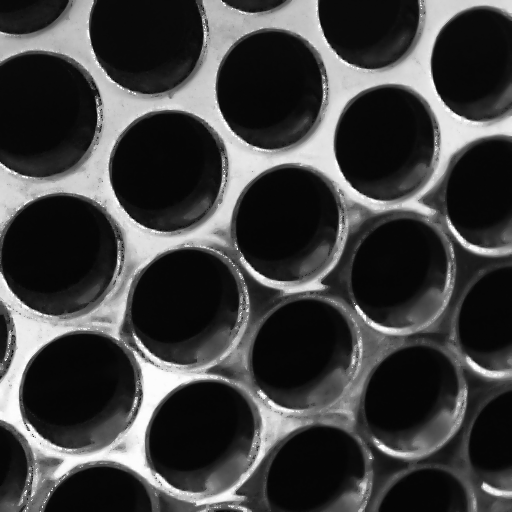
\includegraphics[width=\textwidth]{rec_tv-hub_circles_04.png}
\end{figure}
\end{minipage} %\\[1ex]
\end{center}
\begin{itemize}
\item Reconstruct a randomly corrupted image using only \tb{$30\%$} of the available pixels. \\[0.5ex] 
\item We use $\delta = 0.015$, $\lambda = \delta/8$ and $\gamma = 0.1$, $s = 1$, $\sigma = \frac12$. \\[0.5ex]
\item Results for PGM ($\texttt{tol} = 10^{-2}$): \tp{1181 iter., 24.2 sec.} 
%\item Results for CG-Newton ($\texttt{tol} = 10^{-6}$): \tp{26 iter., 2.30 sec.}   
\end{itemize}
\footlineextra{MDS\,6106 Introduction to Optimization:  L-13}
\end{frame}

%-----------------------------------------------------------------------------------------------------Frame

%-----------------------------------------------------------------------------------------------------Frame

\begin{frame}{Example: Mesh}
\vspace{-1ex}
\begin{center}
\begin{minipage}[c]{0.48\textwidth}
\begin{figure}
\includegraphics[width=\textwidth]{../images/dis_tv_eagle.png}
\end{figure}
\end{minipage}
\hspace{.5ex}
\begin{minipage}[c]{0.48\textwidth}
\begin{figure}
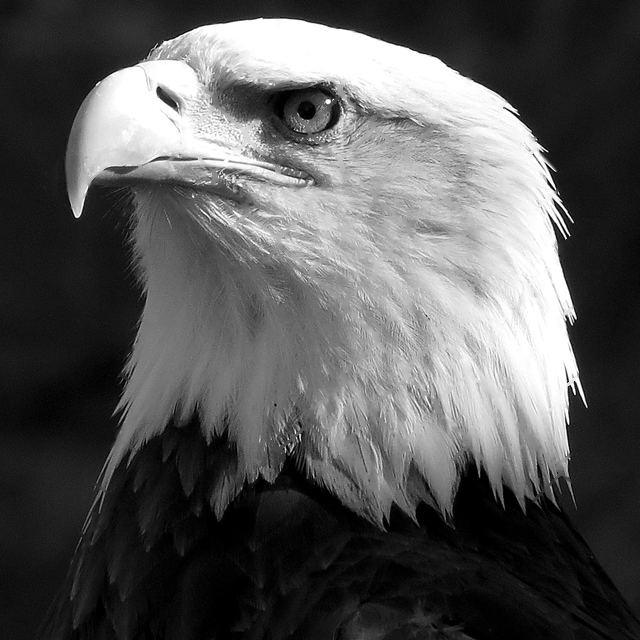
\includegraphics[width=\textwidth]{rec_tv-hub_eagle_04.png}
\end{figure}
\end{minipage} %\\[1ex]
\end{center}
\begin{itemize}
\item[\textcolor{white}{n}] \textcolor{white}{Reconstruct a randomly corrupted image using only {$30\%$} of the available pixels.} \\[0.5ex]
\item We use $\delta = 0.015$, $\lambda = \delta/8$ and $\gamma = 0.1$, $s = 1$, $\sigma = \frac12$. \\[0.5ex]
\item Results for PGM ($\texttt{tol} = 10^{-2}$): \tp{1237 iter., 37.5 sec.}    
%\item Results for CG-Newton ($\texttt{tol} = 10^{-6}$): \tp{19 iter., 3.93 sec.}    
\end{itemize}
\footlineextra{MDS\,6106 Introduction to Optimization:  L-13}
\end{frame}
\end{comment}

%-----------------------------------------------------------------------------------------------------Frame

%-----------------------------------------------------------------------------------------------------Frame

\begin{frame}
\frametitle{\textcolor{cuhkp}{.}}
\bblock
\begin{center}
The Proximal Gradient Method
\end{center}
\eblock
\footlineextra{MDS\,6106 Introduction to Optimization:  L-14}
\end{frame}

%-----------------------------------------------------------------------------------------------------Frame

\begin{frame}
\frametitle{Motivation and Problem Formulation} 

Let us consider the \tp{nonsmooth optimization problem:}
%
\[ \min_x~ \psi(x) = f(x) + \varphi(x) \quad \text{s.t.} \quad x \in \Rn. \vspace{-2ex} \]
%
\begin{itemize}
\item $\varphi : \Rn \to \R$ (or $\varphi : \Rn \to (-\infty,\infty]$) is a \tp{convex} (nonsmooth) function. \\[1ex]
%\item[$\rightsquigarrow$] \tp{Our strategy}: try to mimic the gradient descent method. \\[1.5ex]
\end{itemize}

\tp{Connection to Constrained Problems:} \vspace{1ex}
\begin{itemize}
\item Let us define the \tp{indicator function}: 
\[ \iota_X : \Rn \to (-\infty,+\infty], \quad \iota_X(x) := \begin{cases} 0 & \text{if } x \in X, \\ +\infty & \text{if } x \notin X. \end{cases} \vspace{-1ex}\]
Then, we can write
%
\[ \min_{x \in X}~f(x) \quad \equiv \quad \min_{x \in \Rn}~f(x) + \iota_X(x). \]
\item \tp{Basic Idea}: Replace $\iota_X$ by a general convex mapping $\varphi$. \\[0.5ex]
\item[$\rightsquigarrow$] Transfer techniques and strategies! \\[0.5ex]
\end{itemize}

\footlineextra{MDS\,6106 Introduction to Optimization:  L-14}
\end{frame}
 
%-----------------------------------------------------------------------------------------------------Frame

\begin{frame}
\frametitle{\textcolor{cuhkp}{.}}
\bblock
\begin{center}
Convex Analysis: A Quick Introduction
\end{center}
\eblock
\footlineextra{MDS\,6106 Introduction to Optimization:  L-14}
\end{frame}

%-----------------------------------------------------------------------------------------------------Frame

%-----------------------------------------------------------------------------------------------------Frame

%-----------------------------------------------------------------------------------------------------Frame

%-----------------------------------------------------------------------------------------------------Frame

\begin{frame}
\frametitle{The Convex Subdifferential}
Let us first assume that $\vp$ is differentiable, i.e., we have
%
\[ \vp(y) - \vp(x) \geq \nabla \vp(x)^\top (y-x), \quad \forall~y \in \Rn. \vspace{-2ex} \]
%
\begin{itemize}
\item The tangent $y \mapsto \vp(x) + \nabla \vp(x)^\top (y-x)$ supports $\vp$ at $x$ from below. \\[0.5ex]
\item Generally many such supporting functions might exist! \\[1.5ex]
\item The subdifferential of $\vp$ is defined as the collection of the \tp{subgradients} of these supporting functions. \\[0.5ex]
\end{itemize}

\begin{block}{The Convex Subdifferential} The \tb{subdifferential} of $\vp$ at $x$ is the set
%
\[ \partial \vp(x) := \{ g \in \Rn: \vp(y) - \vp(x) \geq {g}^\top{(y-x)}, \,\, \forall~y\in \Rn\}.\]
%
The elements $g \in \partial \vp(x)$ are called \tb{subgradients} of $\vp$ at $x$. \end{block} 
\footlineextra{MDS\,6106 Introduction to Optimization:  L-14}
\end{frame}

%-----------------------------------------------------------------------------------------------------Frame

\begin{frame}
\frametitle{Illustration: Subdifferential} 

\begin{figure}[t]
\centering
\setlength{\belowcaptionskip}{-6pt}
\begin{tabular}{cc}
\subfloat[Plot of $\vp(x) = |x|$]{
\begin{tikzpicture}[scale=0.63]
\begin{axis}[samples = 200, domain = -1:1,grid]
  \addplot[cuhkpl,very thick] expression { abs(x) };
  %\node[circle,fill=red,scale=0.5] at (axis cs:-2.22,-29.95) {};
  %\node[circle,fill=red,scale=0.5] at (axis cs:0.22,-0.55) {};
  %\node[circle,fill=red,scale=0.5] at (axis cs:2,-13) {};
  %\draw[fill=red] (-2.22,-29.95)  circle (0.5) node[below] {$x_3$};
\end{axis}
\end{tikzpicture}} &
\subfloat[Supporting tangents at $x=0$]{
\begin{tikzpicture}[scale = 0.63 ]
    \begin{axis}[domain=-1:1, samples=200,grid]
     \addplot[cuhkpl,very thick] expression { abs(x) };
     \addplot[cuhkb,thick] expression { -0.2*x };
     \addplot[cuhkb,thick] expression { -0.5*x };
     \addplot[cuhkb,thick] expression { 0.1*x };
     \addplot[cuhkb,thick] expression { 0.7*x };
    \end{axis}
\end{tikzpicture}} 
\end{tabular}
\end{figure}
\tp{Illustration:} \\[1ex] 
\begin{itemize}
\item The absolute value $\vp(x) = |x|$ is differentiable for $x \neq 0$ and we have $\partial \vp(x) = \{+1\}$ if $x > 0$ and $\partial \vp(x) = \{-1\}$ if $x < 0$. In the case $x = 0$, we obtain $\partial \vp(0) = [-1,1]$. \\[2ex]
\end{itemize}

\footlineextra{MDS\,6106 Introduction to Optimization:  L-14}
\end{frame}

%-----------------------------------------------------------------------------------------------------Frame

%-----------------------------------------------------------------------------------------------------Frame

\begin{frame}
\frametitle{Calculus} 
%Next, we present a chain rule for the subdifferential of a composition of convex functions. \vspace{0.5ex}

\begin{block}{Chain Rule for Subdifferentials} Let $f:\Rn \to \R$ and $\vp: \Rm \to \R$ be convex and let $A \in \R^{m \times n}$ be given. Set $\psi(x) : = f(x) + \vp(Ax)$. Then, it holds
%
\[ \partial \psi(x) = \partial f(x) + A^\top \partial \vp(Ax), \quad \forall~x \in \Rn. \vspace{-1ex}\]
\end{block}
\vspace{1ex}
\begin{itemize}
\item Next, we present a connection between classical derivatives and subgradients. \vspace{0.5ex}
\end{itemize}

\begin{block}{Subdifferentiability and Differentiability} Let $\vp:\Rn \to \R$ be convex and let $x \in \Rn$ be given. \\[1ex]
\begin{itemize}
\item Suppose that $\vp$ is (Fr\'{e}chet) differentiable at $x$. Then, we have $\partial\vp(x) = \{\nabla \vp(x)\}$. \\[0.5ex]
\end{itemize}
\end{block}
\footlineextra{MDS\,6106 Introduction to Optimization:  L-14}
\end{frame}

%-----------------------------------------------------------------------------------------------------Frame

%-----------------------------------------------------------------------------------------------------Frame

\begin{frame}
\frametitle{Example: I} 
Calculate the subdifferential of the following mapping: 
%
\[ \vp(x) = \|x\|_2. \]
\vspace{32ex}
\footlineextra{MDS\,6106 Introduction to Optimization:  L-14}
\end{frame}

%-----------------------------------------------------------------------------------------------------Frame

\begin{frame}
\frametitle{Example: II} 
Calculate the subdifferential of the following mapping: 
%
\[ \vp(x) = \max\{0,x\}. \]
\vspace{32ex}
\footlineextra{MDS\,6106 Introduction to Optimization:  L-14}
\end{frame}

%-----------------------------------------------------------------------------------------------------Frame

%-----------------------------------------------------------------------------------------------------Frame

\begin{frame}
\frametitle{\textcolor{cuhkp}{.}}
\bblock
\begin{center}
First-Order Optimality and the Proximity Operator
\end{center}
\eblock
\footlineextra{MDS\,6106 Introduction to Optimization:  L-14}
\end{frame}

%-----------------------------------------------------------------------------------------------------Frame


\begin{frame}
\frametitle{Optimality and Stationary Points}

\begin{block}{First-Order Optimality Conditions}
Let $f$ be cont. diff. and let $\varphi : \Rn \to \R$ be convex. Suppose that $x^*$ is a \tp{local minimizer} of $\min_x \, \psi(x)$, then: \vspace{-1ex}
%
\[ \nabla f(x^*)^\top (x - x^*) + \vp(x) - \vp(x^*) \geq 0 \quad \forall~x \in \Rn. \vspace{-1.5ex} \]
%
\end{block}
\vspace{0.5ex}
\tp{Remarks:} \vspace{1ex}
\begin{itemize}
\item If $f$ is convex, then $x^*$ is a \tb{global sol.} iff the latter cond. holds. \\[1ex]
\item A point $x^*$ with $\nabla f(x^*)^\top(x-x^*) + \vp(x) - \vp(x^*) \geq 0$ for all $x$ is again called \tb{stationary point}. \\[1ex]
\item This condition is equivalent to $-\nabla f(x^*) \in \partial\vp(x^*)$. \\[3ex]
\item[$\rightsquigarrow$] We can now generalize the projection $\mathcal P_X$ in a similar way!
\end{itemize} 

\footlineextra{MDS\,6106 Introduction to Optimization:  L-14}
\end{frame}

%-----------------------------------------------------------------------------------------------------Frame

\begin{frame}
\frametitle{The Proximity Operator}

\begin{block}{The Proximity Operator} %Let $\vp : \Rn \to \R $ be convex. \\[1ex]
\begin{itemize}
\item For every $x \in \Rn$ and $\lambda > 0$, the optimization problem \vspace{-0.5ex}
\[ \min_{y}~\vp(y) + \frac{1}{2\lambda} \|x - y\|^2, \vspace{-0.5ex} \]
has a unique global sol. $x^*$. This minimizer is called the \tb{proximity operator} of $\vp$ at $x$ and we write $x^* = \proxs{\lambda\vp}(x)$. \\[1ex]
%
\item $\proxs{\lambda\vp} : \Rn \to \Rn$ is \tp{Lipschitz cont.} with constant $L=1$. \\[1ex]
\item Let $f :\Rn \to \R$ be $C^1$. Then, $x^*$ is a stationary point iff \vspace{-0.5ex}
%
\[ F_\lambda(x^*) = x^* - \proxs{\lambda\vp}(x^* - \lambda \nabla f(x^*)) = 0 \quad \text{for any} \,\, \lambda > 0. \vspace{-1.5ex} \]
\end{itemize}
\end{block}
\vspace{0.5ex}
The proximity operator can be characterized via:
%
\[ p = \proxs{\lambda\vp}(x) \quad \iff \quad 0 \in \partial \vp(p) + \frac{1}{\lambda}(p-x). \]
%
\footlineextra{MDS\,6106 Introduction to Optimization:  L-14}
\end{frame}

%-----------------------------------------------------------------------------------------------------Frame

%-----------------------------------------------------------------------------------------------------Frame

\begin{frame}
\frametitle{Proximity Operator: Examples}

\tp{Indicator Functions:} \vspace{1ex}
\begin{itemize}
\item Let $X \subseteq \Rn$ be a convex, closed, nonempty set. Then, we have: 
%
\[ \proxs{\lambda \iota_X}(x) = \mathcal P_X(x) \quad \forall~\lambda > 0. \]
%
\end{itemize} 

\tp{$\ell_1$-Norm:} \vspace{1ex}
\begin{itemize}
\item Set $\vp(x) = \mu \|x\|_1$. We have: \vspace{-1ex}
%
\[ [\proxs{\lambda\vp}(x)]_i = \proxs{\lambda\mu|\cdot|}(x_i) =  \begin{cases} x_i - \lambda\mu & \text{if } x_i > \lambda\mu, \\ 0 & \text{if } x_i \in  [-\lambda\mu, \lambda\mu], \\ x_i + \lambda\mu & \text{if } x_i < -\lambda\mu. \end{cases} \]
\end{itemize}

\tp{Maximum-Function:} \vspace{1ex}
\begin{itemize}
\item Set $\vp(x) = \max\{0,x\}$, $x \in \R$. It holds that:
%
\[  \proxs{\lambda\vp}(x) =  \begin{cases} x - \lambda & \text{if } x > \lambda, \\ 0 & \text{if } x \in  [0, \lambda], \\ x & \text{if } x < 0, \end{cases} \quad \text{for all} \quad \lambda > 0. \]
%\item[$\rightsquigarrow$] Many more examples and explicit representations!
\end{itemize} 

\footlineextra{MDS\,6106 Introduction to Optimization:  L-14}
\end{frame}

%-----------------------------------------------------------------------------------------------------Frame

\begin{frame}
\frametitle{Proximity Operator: Illustration}
%\vspace{-5ex}

 \begin{figure}[t]
\centering
\begin{tabular}{cc}
\hspace{-2ex}
\subfloat[$\proxs{\lambda \max\{0,\cdot\}}(x)$ for $\lambda \in \{1,2\}$]{
\begin{tikzpicture}[scale=0.65]
    \begin{axis}[domain=-2:4, samples=200,grid]
     \addplot[blue,thick,dashed] expression { x - max(0,min(1,x)) };
     \addplot[red,thick,dashed] expression { x - max(0,min(2,x)) };
    \end{axis}
\end{tikzpicture}} &
\subfloat[$\proxs{\lambda|\cdot|}$ for $\lambda \in \{1,2\}$ ]{
\begin{tikzpicture}[scale = 0.65]
    \begin{axis}[domain=-3:3, samples=200,grid]
     \addplot[blue,thick,dashed] expression { x - max(-1,min(1,x)) };
     \addplot[red,thick,dashed] expression { x - max(-2,min(2,x)) };
    \end{axis}
\end{tikzpicture}} 
\end{tabular}
\end{figure}
\vspace{2ex}

\begin{itemize}
\item Plot of the proximity operators $\proxs{\lambda \max\{0,\cdot\}}(x)$ and $\proxs{\lambda |\cdot|}(x)$ for different $\lambda$. \\[5ex]
%\item The labels of the $y$-axis are given by $10^{\tilde x^k}$. \\[1ex]
%\item In logarithmic plots, \tp{q-linear convergence} corresponds to \tb{linear behavior} with slope $\log_{10}(0.95)$. 
\end{itemize}
\footlineextra{MDS\,6106 Introduction to Optimization:  L-14}
\end{frame}

%-----------------------------------------------------------------------------------------------------Frame

\begin{frame}
\frametitle{Proximity Operator: Examples}

\tp{$\ell_1$-Norm:} \vspace{1ex}
\begin{itemize}
\item Determine the proximity operator of $\vp(x) = \mu \|x\|_1$. We have: \end{itemize} 
\vspace{32ex}

\footlineextra{MDS\,6106 Introduction to Optimization:  L-14}
\end{frame}


%-----------------------------------------------------------------------------------------------------Frame

\begin{frame}
\frametitle{Proximity Operator: Examples}

\tp{$\ell_2$-Norm:} \vspace{1ex}
\begin{itemize}
\item Determine the proximity operator of $\vp(x) = \mu \|x\|_2$. We have: \end{itemize} 
\vspace{32ex}

\footlineextra{MDS\,6106 Introduction to Optimization:  L-14}
\end{frame}

%-----------------------------------------------------------------------------------------------------Frame

 \begin{frame}
\frametitle{\textcolor{cuhkp}{.}}
\bblock
\begin{center}
The Proximal Gradient Method
\end{center}
\eblock
\footlineextra{MDS\,6106 Introduction to Optimization:  L-14}
\end{frame}

%-----------------------------------------------------------------------------------------------------Frame

\begin{frame}
\frametitle{Descent Direction}

\begin{block}{Descent Directions for Nonsmooth Problems}
Let $x \in \Rn$ and $\lambda > 0$ be given and set $d := - F_\lambda(x)$. Then, we have \vspace{-1ex}
%
\[ \Delta := \nabla f(x)^\top d + \vp(x+d) - \vp(x) \leq - \frac{1}{\lambda} \|d\|^2. \]
%
Suppose that $x$ is \tp{not} a stationary point and choose $\gamma \in (0,1)$. Then, there is $\bar \alpha > 0$ such that \vspace{-1ex}
%
\[ \psi(x + \alpha d) - \psi(x) \leq \gamma \alpha \cdot \Delta \quad \forall~\alpha \in [0, \bar \alpha]. \vspace{-1ex} \]
\end{block}
\vspace{2ex}
\uncover<2->{
\tp{Overall Strategy (As Before):} \vspace{1ex}
\begin{itemize}
\item[$\rightsquigarrow$] Use $d^k = - F_{\lambda_k}(x^k) = \proxs{\lambda_k \vp}(x^k - \lambda_k \nabla f(x^k)) - x^k$ as a descent direction (with some fixed $\lambda_k > 0$). \\[1ex]
\item[$\rightsquigarrow$] Perform \tp{Armijo line-search} to find a step size $\alpha_k$. 
\end{itemize}
}
\footlineextra{MDS\,6106 Introduction to Optimization:  L-14}
\end{frame}

%-----------------------------------------------------------------------------------------------------Frame

\begin{frame}
\frametitle{The Proximal Gradient Method}
\begin{block}{Proximal Gradient Method}    
\begin{itemize}
\item[1.] Initialization: Choose an initial point $x^0 \in \Rn$ and $\sigma, \gamma \in (0,1)$. \\[1ex] 
\end{itemize}
\textbf{For $k = 0,1,... $}: \\[1ex]
\begin{itemize}
\item[2.]{Select $\lambda_k > 0$ and compute $\nabla f(x^k)$ and the new direction $d^k = -F_{\lambda_k}(x^k) = \proxs{\lambda_k \vp}(x^k - \lambda_k \nabla f(x^k)) - x^k$. \\[1ex]} 
\item[3.]{If $\|d^k\| \leq \lambda_k \veps$, then STOP and $x^k$ is the output. \\[1ex]} 
\item[4.]{Choose a maximal step size $\alpha_k \in \{1,\sigma,\sigma^2, ...\} \subset (0,1]$ that satisfies the \tp{Armijo condition} \vspace{-1ex}
\[ \psi(x^k + \alpha_k d^k) - \psi(x^k) \leq \gamma\alpha_k \cdot \Delta_k.\] }
\item[5.]{Set $x^{k+1} = x^k + \alpha_k d^k$.}
\end{itemize} 
\end{block}
\footlineextra{MDS\,6106 Introduction to Optimization:  L-14}
\end{frame}

%-----------------------------------------------------------------------------------------------------Frame

\begin{frame}
\frametitle{Convergence Guarantees}

Let $f : \Rn \to \R$ be $C^1$ and let $\vp : \Rn \to \R$ be convex. Let $\{x^k\}_k$ be generated by the PGM and assume that $\{\lambda_k\}_k$ is \tp{bounded}, i.e.,
%
\[ 0 < \underline\lambda \leq \lambda_k \leq \overline\lambda \quad \forall~k. \]
%
Then, we have: \\[1ex]
\begin{itemize} 
\item The function values $\psi(x^k)$, $k \in \N$, \tb{decrease} and converge to $-\infty$ or some $\psi^* \in \R$. \\[1ex]
%\item In general, $(x^k)_k$ can have \tb{several subsequences} that converge to different accumulation points. \\[0.5ex]
\item \tp{Every accumulation point} $x^*$ of $\{x^k\}_k$ is a \tb{stationary point}. \\[2ex]
\end{itemize}


\uncover<2->{
\tp{Comments:} \vspace{1ex}
\begin{itemize}
\item If $\nabla f$ is \tp{Lipschitz cont.} with constant $L$ and $\lambda_k \in (0,\frac{2}{L})$, then we can use: 
\begin{equation} \label{eq:pm} x^{k+1} = \proxs{\lambda_k\vp}(x^k - \lambda_k \nabla f(x^k)) \end{equation}
\item If $f$ is also \tp{strongly convex}, then $\{x^k\}_k$ converges \tb{q-linearly} to the unique solution $x^*$. \vspace{1ex}
\end{itemize}
%
}
\footlineextra{MDS\,6106 Introduction to Optimization:  L-14}
\end{frame}

%-----------------------------------------------------------------------------------------------------Frame

%-----------------------------------------------------------------------------------------------------Frame

\begin{frame}
\frametitle{Remarks and Discussion}
The update in \eqref{eq:pm} can also be written as:
%
\begin{align*} x^{k+1} & = \proxs{\lambda_k \vp}(x^k - \lambda_k \nabla f(x^k)) \\ & = \argmin_{y \in \Rn}~\vp(y) + \frac{1}{2\lambda_k} \|x^k - \lambda_k \nabla f(x^k) - y\|^2 \\ & = \argmin_{y \in \Rn}~\vp(y) + \nabla f(x^k)^\top (y-x^k) + \frac{1}{2\lambda_k} \|y-x^k\|^2. \end{align*}
%
Hence, the principle idea of PGM can be interpreted as: \\[1ex]
\begin{itemize}
\item We build a \tp{simpler model} of $\psi = \vp + f$ by keeping $\vp$ and by using a quadratic approximation 
\[ f(y) \approx f(x^k) + \nabla f(x^k)^\top (y-x^k) + \frac{1}{2\lambda_k} (y-x^k)^\top(y-x^k) \] 
for the smooth function $f$. \\[0.5ex]
\item The global minimizer of this model is then used to define the next iterate $x^{k+1}$. \\[1ex]
\end{itemize}
\footlineextra{MDS\,6106 Introduction to Optimization:  L-14}
\end{frame}

%-----------------------------------------------------------------------------------------------------Frame

\begin{frame}
\frametitle{Proximal Newton Method}
\tp{Further Remarks:} \\[1ex]
\begin{itemize}
\item This immediately motivates possible extensions of the form: \vspace{2ex}
\end{itemize}
\[ x^{k+1} = \argmin_{y \in \Rn}~\vp(y) + \nabla f(x^k)^\top(y-x^k) + \frac12 (y-x^k)^\top B_k (y-x^k), \]
%
\begin{itemize}
\item[] where $B_k \in \Spp$ is a symmetric, positive definite matrix that can either be the Hessian $\nabla^2 f(x^k)$ or a suitable approximation. \\[2ex]
\end{itemize}

In contrast to the simple PGM step such updates typically do not have closed-form expressions. \\[1ex]
\begin{itemize}
\item[$\rightsquigarrow$] We need to solve a subproblem to calculate $x^{k+1}$. \\[1ex]
\item Methods that are based on this formulation are called \tb{proximal Newton methods}. 
\end{itemize}
\footlineextra{MDS\,6106 Introduction to Optimization:  L-14}
\end{frame}

%-----------------------------------------------------------------------------------------------------Frame

\begin{frame}
\frametitle{\textcolor{cuhkp}{.}}
\bblock
\begin{center}
Proximal Calculus
\end{center}
\eblock
\footlineextra{MDS\,6106 Introduction to Optimization:  L-14}
\end{frame}

%-----------------------------------------------------------------------------------------------------Frame

\begin{frame}
\frametitle{Toolbox: Proximal Calculus - I}

\begin{block}{Translation and Scaling} Let $\lambda > 0$ and $x \in \Rn$ be given. We have: \\[0.5ex]
\begin{itemize}
\item Define $g(\cdot) := \vp(\cdot-b)$, $b \in \Rn$. Then, it follows 
\[ \proxs{\lambda g}(x) = b + \proxs{\lambda \vp}(x-b). \]
\item Define $h(\cdot) := \vp(\cdot/\beta)$, $\beta \neq 0$. Then, it follows 
\[ \proxs{\lambda h}(x) = \beta \cdot \proxs{\lambda \vp / \beta^2}(x / \beta). \vspace{-2ex} \]
\end{itemize}
\end{block}

\begin{block}{Separable Functions} Let $\vp_i : \R \to \R$, $i = 1,...,n$, be a family of convex functions and set $\vp(x) = \sum_{i=1}^n \vp_i(x_i)$. Then, we have
%
\[ [\proxs{\lambda \vp}(x)]_i = \proxs{\lambda \vp_i}(x_i) \quad \forall~i, \quad \lambda > 0. \vspace{-2ex} \]
\end{block}
%
\footlineextra{MDS\,6106 Introduction to Optimization:  L-14}
\end{frame}

%-----------------------------------------------------------------------------------------------------Frame

\begin{frame}
\frametitle{Toolbox: Proximal Calculus - II}

\begin{block}{Composition with a Special Linear Operator} Let $\vp : \R^m \to \R$ be convex and let $x \in \Rn$, $\lambda > 0$ and $A \in \R^{m \times n}$ be given. Suppose $A$ satisfies $AA^\top = I$. \\[1ex] Setting $g(\cdot ) := \vp(A \cdot)$, it holds that:
%
\[ \proxs{\lambda g}(x) = x - A^\top(Ax - \proxs{\lambda \vp}(Ax)). \vspace{-1.5ex} \]
\end{block}
\vspace{1ex}
\tp{Proof: ?} \\[3ex]
\uncover<2->{
\tp{Example:} \vspace{1ex}
\begin{itemize}
\item Let $A \in \R^{m \times n}$ and $b \in \Rm$ be given with $AA^\top = I$. Consider the set $C := \{x : \|Ax - b\| \leq \sigma \}$ and calculate $\mathcal P_C$. \\[1ex]
%
%\item We notice $x \in C \; \iff \; Ax \in K := \{y : y \leq b\}$, i.e., 
%\[ \iota_C(x) = \iota_K(Ax) = (\iota_K \circ A)(x). \]
%\item The set $K$ is much simpler, i.e., we know $\mathcal P_K(y) = \min\{y,b\}$. \\[1ex] 
%\item[$\rightsquigarrow$] We obtain: \\[.5ex]
\end{itemize}
%\[ \mathcal P_C(x) = \proxs{\iota_C}(x) = \proxs{\iota_K \circ A}(x) = A^\top \proxs{\iota_K}(Ax) = A^\top \mathcal P_K(Ax). \] 
}
\footlineextra{MDS\,6106 Introduction to Optimization:  L-14}
\end{frame}

%-----------------------------------------------------------------------------------------------------Frame

%-----------------------------------------------------------------------------------------------------Frame

\begin{frame}
\frametitle{\textcolor{cuhkp}{.}}
\bblock
\begin{center}
The Accelerated Proximal Gradient Method
\end{center}
\eblock
\footlineextra{MDS\,6106 Introduction to Optimization:  L-14}
\end{frame}

%-----------------------------------------------------------------------------------------------------Frame 

\begin{frame}
\frametitle{Let's Accelerate!}

It is possible to combine the discussed \tb{acceleration techniques} and the proximal gradient method under the assumption that $f$ is a convex mapping. \\[1.5ex]

In principle, the acceleration mechanism is identical to the one we already discussed! \\[1.5ex]

\begin{itemize}
\item We first perform an \tp{extrapolation step }
%
\[ y^{k+1} = x^k + \beta_k (x^k - x^{k-1}), \quad\quad \beta_k > 0 \]
%
to approximate and extrapolate the next iterate $y^{k+1} \approx x^{k+1}$. \\[1ex]
\item Afterwards we compute a proximal gradient step based on the predicted information $y^{k+1}$.  
\end{itemize}

\footlineextra{MDS\,6106 Introduction to Optimization:  L-14}
\end{frame}

%-----------------------------------------------------------------------------------------------------Frame 

\begin{frame}
\frametitle{The Accelerated Proximal Gradient Method}
\begin{block}{Accelerated Proximal Gradient Method}    
\begin{itemize}
\item[1.] Initialization: Choose a point $x^0 \in \Rn$ and set $x^{-1} = x^0$. \\[1ex] 
\end{itemize}
\textbf{For $k = 0,1,... $}: \\[1ex]
\begin{itemize}
\item[2.] Select an extrapolation parameter $\beta_k$ and compute the step $y^{k+1} = x^k + \beta_k (x^k - x^{k-1})$. \\[1.5ex]
\item[3.]{Select $\lambda_k > 0$ and set $x^{k+1} = \proxs{\lambda_k\vp}(y^{k+1} - \lambda_k \nabla f(y^{k+1}))$. \\[1ex]} 
\end{itemize} 
\end{block}
\vspace{1.5ex}
\begin{itemize}
\item For special choices of $\beta_k$ and \tp{$\lambda_k = \bar \lambda \in (0,\frac1L]$}, we can show:
% 
\[ \psi(x^k) - \psi(x^*) \leq \frac{2 \|x^0 - x^*\|^2}{\bar\lambda(k+1)^{{2}}} \quad \forall~k \in \N,\]
%
where $x^*$ is a solution of the problem $\min_x \, \psi(x)$. \end{itemize}
\footlineextra{MDS\,6106 Introduction to Optimization:  L-14}
\end{frame}

%-----------------------------------------------------------------------------------------------------Frame

%-----------------------------------------------------------------------------------------------------Frame 

%-----------------------------------------------------------------------------------------------------Frame 

\begin{frame}
\frametitle{Remarks and Choices of $\beta_k$}

As in the smooth case, we can utilize the choices $\beta_k = \frac{k-2}{k+1}$ or
%
\[ t_k = \frac{1+\sqrt{1+4t_{k-1}^2}}{2}, \quad \beta_k = \frac{t_{k-1}-1}{t_k}, \quad t_{-1} = t_0 = 1. \]
%
\\[3ex]
%
If the Lipschitz constant $L$ is unknown, then the step size $\lambda_k$ can be determined by the following line search procedure: \\[1ex]
\begin{itemize}
\item Choose $\eta \in (0,1)$. \\[0.5ex]
\item Set $\lambda_k = \lambda_{k-1}$ and $x^{k+1} = \proxs{\lambda_k \vp}(y^{k+1} - \lambda_k \nabla f(y^{k+1}))$. \\[0.5ex]
\item \texttt{while} {\scriptsize$f(x^{k+1}) > f(y^{k+1}) + \nabla f(y^{k+1})^\top (x^{k+1} - y^{k+1}) + \frac{\|x^{k+1} - y^{k+1}\|^2}{2\lambda_k} $} \texttt{do}: \\[0.5ex]

Set $\lambda_k = \eta \lambda_k$ and calc. $x^{k+1} = \proxs{\lambda_k \vp}(y^{k+1} - \lambda_k \nabla f(y^{k+1}))$. 
\end{itemize}

\footlineextra{MDS\,6106 Introduction to Optimization:  L-14}
\end{frame}

%-----------------------------------------------------------------------------------------------------Frame 

\begin{frame}
\frametitle{\textcolor{cuhkp}{.}}
\bblock
\begin{center}
Numerical Experiment: Sparse Reconstruction
\end{center}
\eblock
\footlineextra{MDS\,6106 Introduction to Optimization:  L-14}
\end{frame}

%-----------------------------------------------------------------------------------------------------Frame

\begin{frame}
\frametitle{Numerical Example}

We consider the $\ell_1$-optimization problem
%
\[ \min_x~\psi(x) = \frac12 \|Ax - b\|^2 + \mu \|x\|_1. \]
%
The data is generated as follows: \\[0.5ex]
\begin{itemize}
\item We set $\texttt{m} = 300$, $\texttt{n} = 3000$, $\texttt{s} = 30$ and create an index mask $\texttt{mask} = \texttt{randperm(n,s)}$. We generate a sparse signal $x^*$ via
%
\[ x^* = \texttt{zeros(n,1)}, \quad x^*(\texttt{mask}) = \texttt{randn(s,1)}. \]
%
\item[$\rightsquigarrow$] $x^*$ has only 30 nonzero randomly chosen components. \\[0.5ex]
\item We choose \texttt{A} = \texttt{randn(m,n)} and generate the measurement $b$ via $\texttt{b} = \texttt{A} \cdot x^* + 0.01\cdot \texttt{randn(m,1)}$. \\[0.5ex]
\item[$\rightsquigarrow$] The goal is to reconstruct the signal $x^*$ from the much smaller measurements $b$ via solving the $\ell_1$-problem. \\[0.5ex]
\item The Lipschitz constant of $\nabla f$ is given by $L = \lambda_{\max}(A^\top A)$. %All other parameter are set as usual.
\end{itemize}
\footlineextra{MDS\,6106 Introduction to Optimization:  L-14}
\end{frame}

%-----------------------------------------------------------------------------------------------------Frame

\begin{frame}
\frametitle{Numerical Comparison}

We consider the accelerated proximal gradient method (APGM) with the following setups: \\[1ex]
\begin{itemize}
\item[1.] We set $\beta_k = (t_{k-1}-1)t_k^{-1}$, $t_k = 0.5(1+\sqrt{1+4t_{k-1}^2})$, and $\lambda_k \equiv \bar\lambda = 1/L$; \\[0.5ex]
\item[2.] Same strategy for $\beta_k$ and $\lambda_k$ with restart $t_{k-1} = t_k = 1$ after each $50$ iterations; \\[0.5ex]
\item[3.] Alternative extrapolation strategy: $\beta_k = \frac{k-2}{k+1}$ and $\lambda_k = 1/L$; \\[2.5ex]
\end{itemize}

We compare APGM with: \\[1ex]
\begin{itemize}
\item The basic proximal gradient method with quasi-Armijo line search and $\gamma = 0.1$, $s = 1$, $\sigma = 0.5$. \\[1.5ex] 
\end{itemize}

We use $x^0 = 0$ and $\mu = 5$. The tolerance is set to $\texttt{tol} = 10^{-8}$.
\footlineextra{MDS\,6106 Introduction to Optimization:  L-14}
\end{frame}

%-----------------------------------------------------------------------------------------------------Frame 

\begin{frame}
\frametitle{Numerical Results}

\begin{figure}[th]
\begin{adjustwidth}{-1in}{-1in}% adjust the L and R margins by 1 inch
\centering
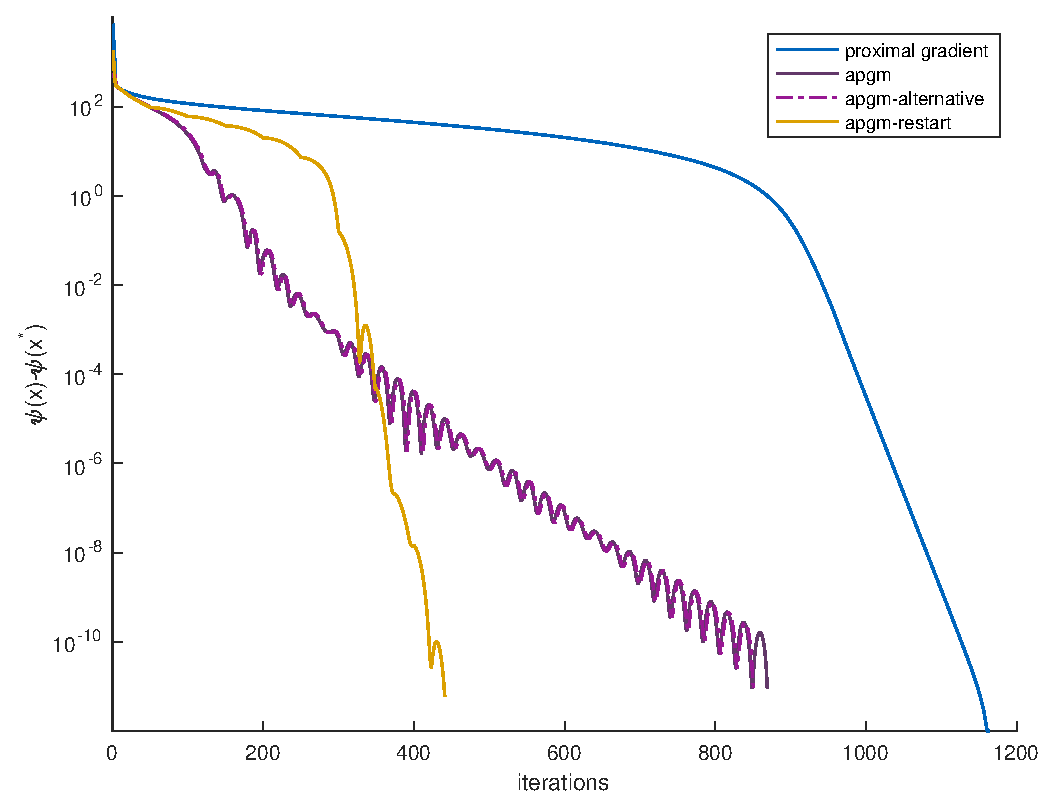
\includegraphics[width=0.8\textwidth]{demo_pd_l1.eps} 
\end{adjustwidth}
%\caption{Illustration of Example 3.9}
%trim={1.5cm 1cm 1.5cm 0.5cm},clip
%\label{fig:example-8}
\end{figure}

\footlineextra{MDS\,6106 Introduction to Optimization:  L-14}
\end{frame}

%-----------------------------------------------------------------------------------------------------Frame 

\begin{frame}
\frametitle{Comparison: Sparsity Pattern}

\begin{figure}[th]
\begin{adjustwidth}{-1in}{-1in}% adjust the L and R margins by 1 inch
\centering
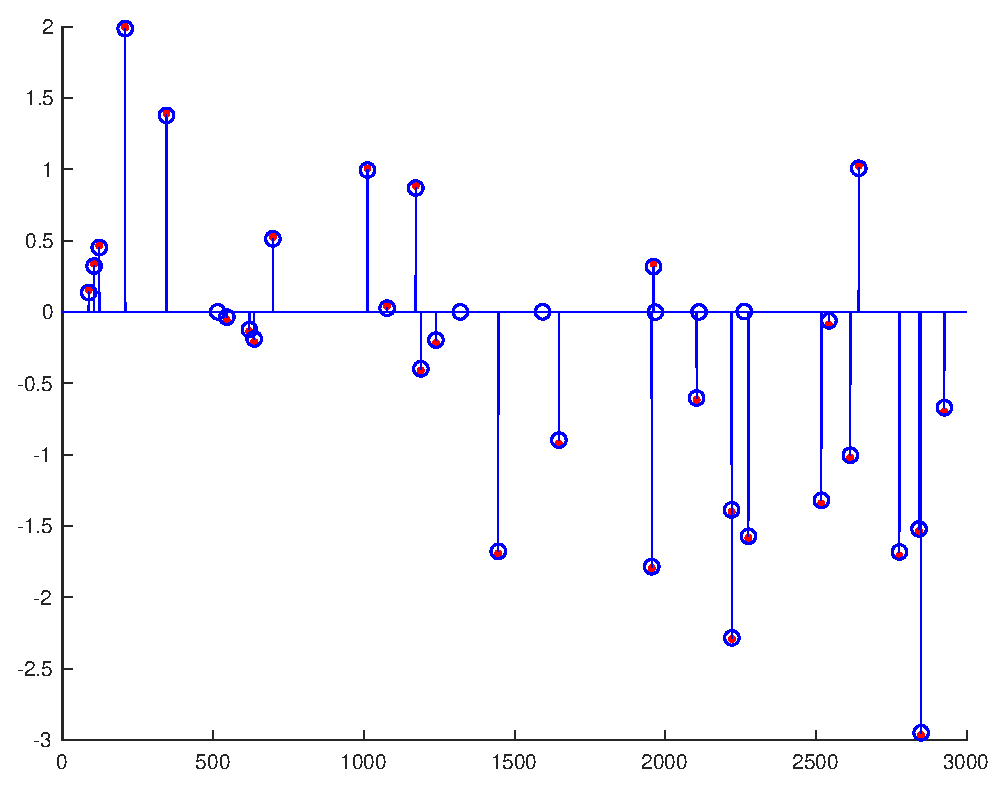
\includegraphics[width=0.8\textwidth]{demo_apgm_sparsity.eps} 
\end{adjustwidth}
%\caption{Illustration of Example 3.9}
%trim={1.5cm 1cm 1.5cm 0.5cm},clip
%\label{fig:example-8}
\end{figure}

\footlineextra{MDS\,6106 Introduction to Optimization:  L-14}
\end{frame}

%-----------------------------------------------------------------------------------------------------Frame

\begin{frame}
\frametitle{Comparison: Sparsity Pattern -- $\vp(x) = \frac{\mu}{2}\|x\|^2$}

\begin{figure}[th]
\begin{adjustwidth}{-1in}{-1in}% adjust the L and R margins by 1 inch
\centering
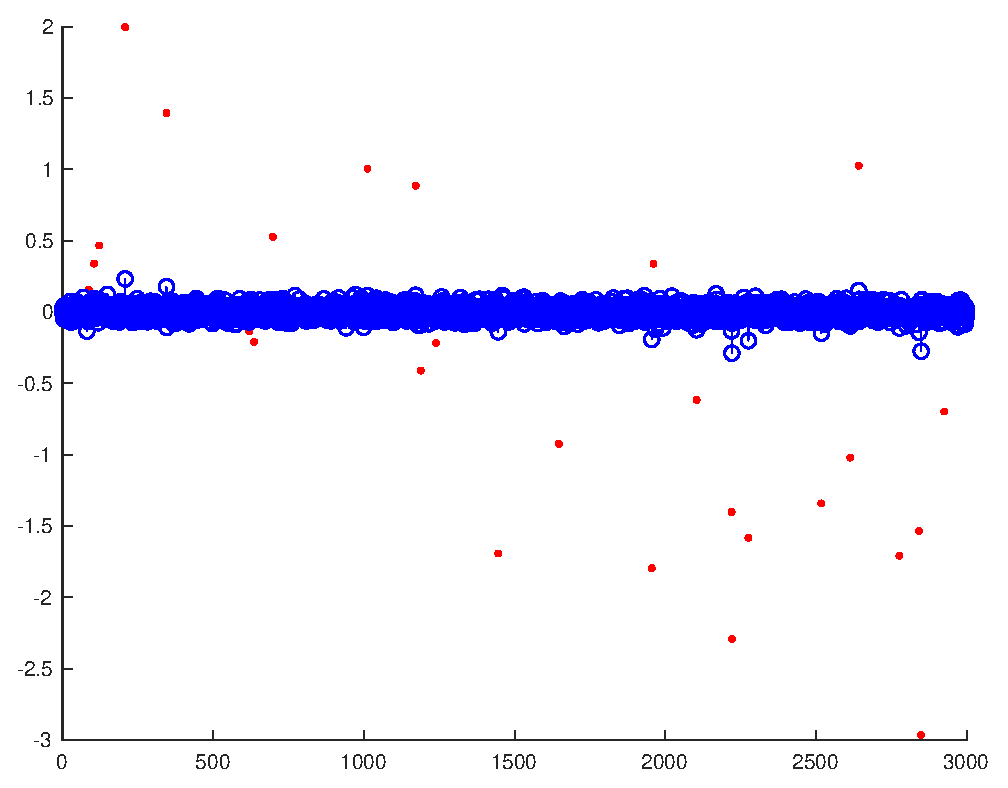
\includegraphics[width=0.8\textwidth]{demo_apgm_ell2.eps} 
\end{adjustwidth}
%\caption{Illustration of Example 3.9}
%trim={1.5cm 1cm 1.5cm 0.5cm},clip
%\label{fig:example-8}
\end{figure}

\footlineextra{MDS\,6106 Introduction to Optimization:  L-14}
\end{frame}

%-----------------------------------------------------------------------------------------------------Frame

\begin{frame}
\frametitle{How to Apply the Proximal Gradient Method?}
\vspace*{-.5ex}
%\begin{block}{\vspace*{-3ex}}
\hspace*{\fill}\begin{minipage}{10cm}
\bblock
%\vspace*{-2.9ex}
\vspace*{1ex}
\hspace*{\fill}
We want to solve: \quad $\displaystyle \min_x~\psi(x)$ %\text{where}\quad M\in\partial F^\Lambda(x)$,
\hspace*{\fill} 
\vspace*{0.3ex}
%\vspace*{-3.7ex}
\eblock
\end{minipage}\hspace*{\fill} \\
\vspace{2ex}

\begin{itemize}
\item Identify the structure of the problem. Can $\psi$ be written as 
\[ \psi = f + \varphi \]
where $f$ is \tp{smooth} and $\varphi$ is \tp{convex}? \\[1ex]
\item Is the problem constrained with \tp{convex constraints} $x \in C$? \\[1ex]
\end{itemize}

\uncover<2->{
\tp{Yes $\rightsquigarrow$ Apply Proximal/Projected Gradient Method:} \vspace{.5ex}
\begin{itemize}
\item Expressions for $\proxs{\lambda\varphi}$ or $\mathcal P_C$ often exist if $\varphi$ or $C$ are \tp{simple}! \\[1ex]
\item Identify the ``\tp{simple structure}'' in $\varphi$ and $C$ and try to use the \tb{proximal calculus}. \\[1ex]
\end{itemize}
}

\uncover<3->{
\tp{No $\rightsquigarrow$ $\ldots$:} \vspace{.5ex}
\begin{itemize}
\item If $\varphi \equiv 0$ or $C = \Rn$, an \tp{unconstrained optimization method} can be applied (gradient, Newton, BFGS).  \\[1ex]
\end{itemize}
}
\footlineextra{MDS\,6106 Introduction to Optimization:  L-14}
\end{frame}

%-----------------------------------------------------------------------------------------------------Frame

\begin{frame}
\frametitle{\textcolor{cuhkp}{.}}
\bblock
\begin{center}
Bonus: Alternating Direction Method of Multiplier
\end{center}
\eblock
\footlineextra{MDS\,6106 Introduction to Optimization:  L-14}
\end{frame}

%-----------------------------------------------------------------------------------------------------Frame

\begin{frame}
\frametitle{Background}
We now discuss an algorithm that can also be applied to more complicated models. \\[1ex] 

The starting point for the so-called \tb{alternating direction method of multipliers} or \tb{ADMM} are minimization problems of the form:
%
\begin{equation} \label{eq:admm} \min_{x \in \Rn}~f(x) + g(Ax), \end{equation}
%
\begin{itemize}
\item $A$ is a given $m \times n$ matrix. \\[0.5ex]
\item  $f : \Rn \to \R$,  $g : \Rm \to \R$ are convex functions (or constraint functions: $\iota_X$). \\[1.5ex]
\end{itemize}

\tp{Observation:} \\[1ex]
\begin{itemize}
\item[$\rightsquigarrow$] Both $f$ and $g$ can be nonsmooth! 
\end{itemize}
\footlineextra{MDS\,6106 Introduction to Optimization:  L-14}
\end{frame}

%-----------------------------------------------------------------------------------------------------Frame

\begin{frame}
\frametitle{Derivation}
We convert this problem to the equivalent constrained problem 
%
\[ \min~f(x) + g(y) \quad x \in \Rn, \quad y \in \Rm, \quad Ax - y = 0. \]
%
 The associated \tp{augmented Lagrangian function} is given by:
 %
 \[ L_\sigma(x,y,\lambda) = f(x) + g(y) + \lambda^\top (Ax - y) + \frac{\sigma}{2} \|Ax - y\|^2. \]
 %
 The ADMM first minimizes the augmented Lagrangian w.r.t. $x$, then w.r.t. $y$, and finally performs a multiplier update: 
 %
 \bblock \vspace{-4ex}
 \begin{align*} x^{k+1} & \in \argmin_{x \in \Rn}~L_\sigma(x,y^k,\lambda^k) \\ y^{k+1} & \in \argmin_{y \in \Rm}~L_\sigma(x^{k+1},y,\lambda^k) \\ \lambda^{k+1} & = \lambda^k + \gamma\sigma(Ax^{k+1} - y^{k+1}),\end{align*} \vspace{-4ex} 
 \eblock
 %
where $\gamma \in (0,(1+\sqrt{5})/2)$. \\[1ex]
\footlineextra{MDS\,6106 Introduction to Optimization:  L-14}
\end{frame}

%-----------------------------------------------------------------------------------------------------Frame

\begin{frame}
\frametitle{Derivation and Discussion}
The minimization with respect to $y$ can also be written more compactly
 %
 \begin{align*} y^{k+1} &= \argmin_{y \in \Rm}~g(y) + (\lambda^k)^\top (Ax^{k+1} - y) + \frac{\sigma}{2} \|Ax^{k+1} - y\|^2 \\ & = \proxs{g/\sigma}(Ax^{k+1} + \sigma^{-1}\lambda^k). \end{align*}
 %
The penalty parameter $\sigma$ is typically kept constant in ADMM. \\[1ex]

\tp{Observations:} \\[1ex]
\begin{itemize}
\item Very simple procedure that performs \tp{separate minimization} w.r.t. $x$ and  $y$. \\[0.5ex]
\item[$\rightsquigarrow$] \tp{Key Modeling Technique:} (Re-)Formulate the problem such that the subproblems are easy to solve ($\rightsquigarrow$ proximal calculus). \\[1.5ex] 
\end{itemize}
%Before presenting convergence results and a more refined version of the algorithm, we consider several applications and examples. 
\footlineextra{MDS\,6106 Introduction to Optimization:  L-14}
\end{frame}

%-----------------------------------------------------------------------------------------------------Frame

\begin{frame}
\frametitle{\textcolor{cuhkp}{.}}
\bblock
\begin{center}
Application: Support Vector Machines
\end{center}
\eblock
\footlineextra{MDS\,6106 Introduction to Optimization:  L-14}
\end{frame}

%-----------------------------------------------------------------------------------------------------Frame

\begin{frame}
\frametitle{Example: Sparse Recovery}
We consider the \tp{$\ell_1$-optimization problem}
%
\[ \min_{x}~\frac12 \|Ax-b\|^2 + \mu \|x\|_1, \]
%
where $A \in \R^{m \times n}$, $b \in \Rm$, and $\mu > 0$ are given. \\[30ex]
\footlineextra{MDS\,6106 Introduction to Optimization:  L-14}
\end{frame}

%-----------------------------------------------------------------------------------------------------Frame

%-----------------------------------------------------------------------------------------------------Frame

\begin{comment}
\begin{frame}{An Alternative Formulation}
Notice that we can also rewrite problem \eqref{eq:admm} in the following way: 
%
\begin{equation} \label{eq:prob3} \min_{x,y,z}~f(z) + g(y) \quad \text{s.t.} \quad Ax - y = 0, \quad x - z = 0. \end{equation}
%
This formulation still fits our ADMM-framework and the aug- mented Lagrangian is given by:
%
\begin{align*} L_\sigma(x,y,z,\lambda_1,\lambda_2) & = f(z) + g(y) + \lambda_1^\top (Ax-y) + \lambda_2^\top (x-z) \\ & \hspace{4ex} + \frac{\sigma}{2} \|Ax-y\|^2 + \frac{\sigma}{2} \|x-z\|^2. \end{align*}
%
\begin{itemize}
\item[$\rightsquigarrow$] The additional auxiliary variable $z$ allows to further decouple the problem! (At the cost of a larger number of primal and dual variables). 
\end{itemize}
\footlineextra{MDS\,6106 Introduction to Optimization:  L-14}
\end{frame}
\end{comment}

%-----------------------------------------------------------------------------------------------------Frame

\begin{comment}
\begin{frame}{The Alternative ADMM-Scheme}
The full ADMM-scheme for the alternative formulation \eqref{eq:prob3} is then given by: \\[2ex]
\bblock \vspace{-4ex}
\begin{align*} x^{k+1} & = [I + A^\top A]^{-1} (A^\top[y^k - \sigma^{-1}\lambda_1^k] + z^k - \sigma^{-1}\lambda_2^k) \\[0.5ex] y^{k+1} & = \proxs{g/\sigma}(Ax^{k+1} + \sigma^{-1}\lambda_1^k) \\ z^{k+1} & = \proxs{f/\sigma}(x^{k+1} + \sigma^{-1}\lambda_2^k) \\[0.5ex] \lambda_1^{k+1} & = \lambda_1^k + \gamma\sigma (Ax^{k+1} - y^{k+1}) \\[0.5ex] \lambda^{k+1}_2 & = \lambda_2^k + \gamma\sigma(x^{k+1} - z^{k+1}). \end{align*} \vspace{-3.5ex}
\eblock 

\footlineextra{MDS\,6106 Introduction to Optimization:  L-14}
\end{frame}
\end{comment}

%-----------------------------------------------------------------------------------------------------Frame

\begin{frame}
\frametitle{\textcolor{cuhkp}{.}}
\bblock
\begin{center}
Application: Support Vector Machines
\end{center}
\eblock
\footlineextra{MDS\,6106 Introduction to Optimization:  L-14}
\end{frame}

%-----------------------------------------------------------------------------------------------------Frame

\begin{frame}{Example: Support Vector Machines}
\tp{Given}: $m$ data points $a_1,a_2,...,a_m \in \Rn$ with \tb{labels} $b_i \in \{-1,1\}$. \\[1ex]

\tp{Task}: Find a hyperplane $\ell(a) := a^\top x + y$ defined by $(x,y) \in \R^{n +1}$ separating the datapoints such that: \vspace{-1ex}
\[ b_i = \begin{cases} +1 & \text{if } \ell(a_i) > 0, \\ -1 & \text{if } \ell(a_i) \leq 0. \end{cases}  \]

We consider the SVM-model: \\[1.5ex]
\vspace*{-1ex}
%\begin{block}{\vspace*{-3ex}}
\hspace*{\fill}\begin{minipage}{10cm}
\bblock
%\vspace*{-2.9ex}
\vspace*{0.6ex}
\hspace*{\fill}
$\displaystyle \min_{x,y} \quad \frac{\lambda}{2} \|x\|^2  +  {\sum}_{i=1}^m \max\{0, 1 - b_i(a_i^\top x + y) \}, \quad \lambda > 0.$ \vspace{-0.5ex} %\text{where}\quad M\in\partial F^\Lambda(x)$,
\hspace*{\fill} 
\vspace*{0.3ex}
%\vspace*{-3.7ex}
\eblock
\end{minipage}\hspace*{\fill} \\
\vspace{3ex}
\begin{itemize}
\item We want to apply ADMM to solve this problem. 
\end{itemize}
\footlineextra{MDS\,6106 Introduction to Optimization:  L-14}
\end{frame}

%-----------------------------------------------------------------------------------------------------Frame

%-----------------------------------------------------------------------------------------------------Frame

%-----------------------------------------------------------------------------------------------------Frame

\begin{frame}
\frametitle{\textcolor{cuhkp}{.}}
\bblock
\begin{center}
Semi-Proximal Alternating Direction Method of Multiplier
\end{center}
\eblock
\footlineextra{MDS\,6106 Introduction to Optimization:  L-14}
\end{frame}

%-----------------------------------------------------------------------------------------------------Frame

\begin{frame}{Semi-Proximal ADMM}

We now analyze a more general version of ADMM. \\[1ex]
\begin{itemize}
\item We add a quadratic proximity term to the objective function of each subproblem in ADMM. \\[0.5ex]
\item Let $S \in \mathbb{S}_+^n$, $T \in \mathbb{S}_+^m$ be given. We set $\|x\|^2_S = x^\top S x$ and $\|y\|^2_T = y^\top T y$. \\[1.5ex]
\end{itemize}

We now consider the so-called \tp{semi-proximal ADMM}:

\begin{block}{sp-ADMM}    
\begin{itemize}
\item[1.] Initialization:~Choose an initial points $x^0 \in \Rn$, $y^0, \lambda^0 \in \Rm$, and $\sigma > 0$, $\gamma \in (0,(1+\sqrt{5})/2)$. \\[0.5ex] 
\end{itemize}
{Perform the following updates:} \\[0.5ex]
\begin{itemize}
\item[2.] {\small $x^{k+1} \in \argmin_{x \in \Rn}~f(x) + \frac{\sigma}{2}\|Ax - y^k + \sigma^{-1}\lambda^k\|^2 + \frac12 \|x-x^k\|_S^2$.} \\ [0.5ex]
\item[3.] {\small $y^{k+1} \in \argmin_{y \in \Rm}~g(y) + \frac{\sigma}{2}\|Ax^{k+1}  - y + \sigma^{-1}\lambda^k\|^2 + \frac12 \|y-y^k\|_T^2$.} \\[0.5ex] 
\item[4.] {\small$\lambda^{k+1} = \lambda^k + \gamma\sigma (Ax^{k+1}-y^{k+1})$.} 
\end{itemize}
\end{block}
%
\footlineextra{MDS\,6106 Introduction to Optimization:  L-14}
\end{frame}

%-----------------------------------------------------------------------------------------------------Frame

\begin{frame}{Discussion}
\tp{Important Observation:} \\[1ex]
\begin{itemize}
\item The minimization in step 2 can be considerably simplified by choosing $S = \tau I - \sigma A^\top A$ with $\tau \geq \sigma \lambda_{\max}(A^\top A)$. \\[1.5ex]
\end{itemize} 
%
Then, we have $S \in \mathbb{S}^+_n$ and the $x$-step can be simplified as follows: \\[1ex]
%
\[ f(x) + \frac{\sigma}{2}\|Ax - y^k + \sigma^{-1}\lambda^k\|^2 + \frac12 \|x-x^k\|_S^2  \; = \; ... \]
%
\vspace{15ex}
%\begin{align*}
%f(x) + \frac{\sigma}{2}\|Ax - y^k + \sigma^{-1}\lambda^k\|^2 + \frac12 \|x-x^k\|_S^2 & \\ & \hspace{-40ex} = f(x) + \frac{\sigma}{2} \|A(x-x^k)\|^2 + \sigma \iprod{A(x-x^k)}{Ax^k - y^k +\sigma^{-1}\lambda^k} + \frac12 \|x-x^k\|_S^2 + \text{cons.} \\ & \hspace{-40ex} = f(x) + \iprod{A(x-x^k)}{\sigma (Ax^k - y^k) + \lambda^k} + \frac{\tau}{2} \|x-x^k\|^2 + \text{cons.} \\ & \hspace{-40ex} = f(x) + \frac{\tau}{2}\|x - x^k + \frac{\sigma}{\tau} A^\top[Ax^k - y^k +\sigma^{-1}\lambda^k] \|^2 + \text{cons.} \end{align*}
%
\footlineextra{MDS\,6106 Introduction to Optimization:  L-14}
\end{frame}

%-----------------------------------------------------------------------------------------------------Frame

\begin{frame}{The Linearized Semi-Proximal ADMM}
Thus, with this choice of $S$ and setting $T = 0$, step 2 and 3 in sp-ADMM can be expressed explicitly via: \\[1.5ex]
%
\bblock \vspace{-4ex}
\begin{align*}
x^{k+1} &= \proxs{f/\tau}(x^k - \frac{\sigma}{\tau} A^\top[Ax^k - y^k +\sigma^{-1}\lambda^k]) \\ y^{k+1} & = \proxs{g/\sigma}(Ax^{k+1} + \sigma^{-1}\lambda^k). \end{align*}  \vspace{-3.5ex}
\eblock

\tp{Remark:} \\[1ex]
\begin{itemize}
\item This special version of ADMM is called \tp{linearized semi- proximal linearized ADMM}. \\[1ex] 
\item[$\rightsquigarrow$] In the updates in step 2 and 3, we actually linearize the original quadratic terms and add a quadratic proximity term. 
\end{itemize}

\footlineextra{MDS\,6106 Introduction to Optimization:  L-14}
\end{frame}

%-----------------------------------------------------------------------------------------------------Frame

\begin{frame}
\frametitle{\textcolor{cuhkp}{.}}
\bblock
\begin{center}
Merry Christmas!
\end{center}
\eblock
\footlineextra{MDS\,6106 Introduction to Optimization:  L-14}
\end{frame}

%-----------------------------------------------------------------------------------------------------Frame


\end{document}
